\subsection{Data Types}
\label{sec:data_types}

The \sunpypkg package provides two core data types that are designed to provide a general, standard, and consistent interface for loading and representing solar data across different instruments and missions.
The two core data types currently supported in \sunpypkg are handled by \Timeseries and \Map, objects that support 1D temporal data and 2D image data, respectively.
The purpose of these core classes is to standardize data structures regardless of the data source (e.g., observational data from independent instruments).
The classes maintain a consistent interface for accessing data attributes such as the data array itself as well as the metadata and relevant units.
This arrangement allows for an easier workflow in the analysis of solar data observations.
These core classes also include functionality for data manipulation and data visualization.
This section provides an overview of the \Timeseries and \Map data types.

\subsubsection{\Timeseries}
\label{sec:timeseries}
Many observations in the field of solar physics consist of spatially-integrated measurements as a function of time.
For example, the X-Ray Sensor (XRS) instrument aboard the Geostationary Operational Environmental Satellite (GOES), which is used as the classification standard for solar flares, continuously measures the disk-integrated X-ray flux as a function of time in two broadband channels.
The \Timeseries class aims to accommodate such solar time series data.

\Timeseries allows users to load time series data from a variety of solar instruments with appropriate units and time scales (see \autoref{sec:units}).
 A user can create a \Timeseries object either from data files stored locally (e.g., observational datasets acquired through \Fido, see \autoref{sec:fido}), or manually from custom time series data.
 The data array, metadata, and units data are all stored as attributes in the \Timeseries class.

Functionality is also provided for the manipulation of time series, including: adding, updating, truncating, resampling, and combining data within a \Timeseries or combining multiple \Timeseries together.
\Timeseries also has built-in visualization methods to allow for easy inspection.
An example of a \Timeseries created from GOES XRS observations of a solar flare is shown in \autoref{fig:timeseries_example}.

\begin{figure}
    \centering
    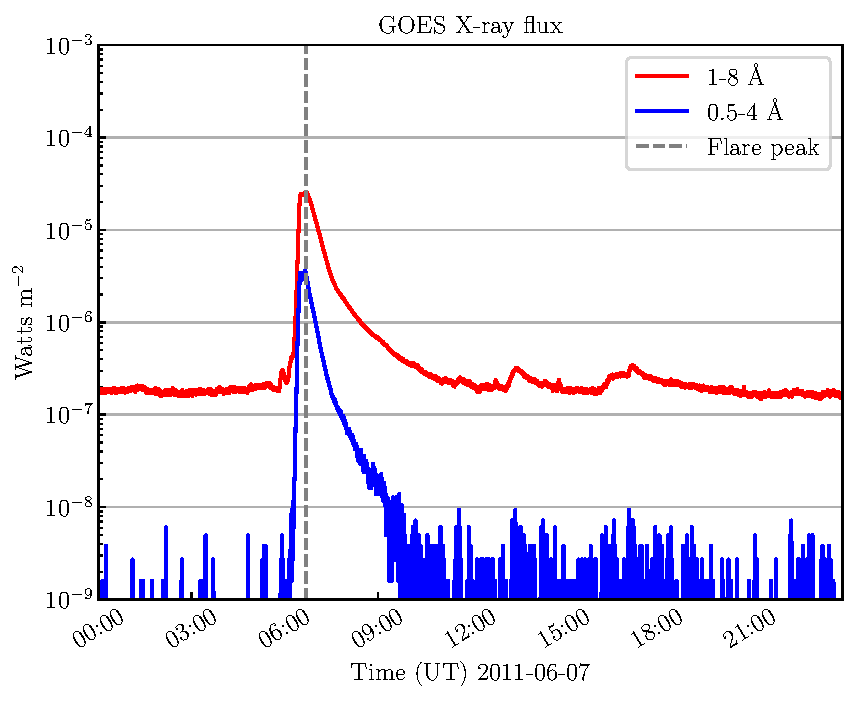
\includegraphics[width=0.55\textwidth]{figures/timeseries_example.pdf}
    \caption{An example of a GOES XRS \Timeseries visualization over 24 hours. The two colors represent the two broadband channels; 1--8~\AA\ (red) and 0.5--4~\AA\ (blue).  The sharp increase in flux at 06:33 UT is a solar flare and the grey dashed line indicates the time of the peak provided by the HEK.}
    \label{fig:timeseries_example}
\end{figure}

\Timeseries currently supports the data sources listed in \autoref{tab:instruments} in addition to indices of solar activity from the National Oceanic and Atmospheric (NOAA) Space Weather Prediction Center that track the solar cycle and its predicted progression. Due to its flexible data structure, it is straightforward to add additional instruments and data sources to the \Timeseries object.

%%%%%%%%%%%%%%%% TABLE %%%%%%%%%%%%%%%%%%%
\begin{table}
\begin{center}
\begin{tabular}{|p{12cm}|c|c|}
\hline
& \\
\textbf{Supported by \Timeseries}& \textbf{Instrument reference}\\
\hline
\hline
\textit{Geostationary Operational Environmental Satellite} (GOES) X-Ray Sensor (XRS) & \citet{garcia94, hanser96} \\
\hline
\textit{Fermi} Gamma-ray Burst Monitor (GBM) &  \citet{meegan2009fermi} \\
\hline
\textit{Nobeyama Radioheliograph} (NoRH) & \citet{nakajima1994nobeyama} \\
\hline
\textit{PRoject for Onboard Autonomy} (PROBA2) Large Yield Radiometer (LYRA) & \citet{dominique2013lyra} \\
\hline
\textit{Solar Dynamics Observatory} (SDO) EUV Variability Experiment (EVE) & \citet{woods2010extreme}  \\
\hline
\textit{Reuven Ramaty High Energy Solar Spectroscopic Imager} (RHESSI) & \citet{lin2002reuven} \\
\hline
 & \\
\textbf{Supported by \Map} & \textbf{Instrument reference} \\
\hline
\hline
\textit{COronal Solar Magnetism Observatory} (COSMO) K-coronagraph (K-Cor) & \citet{dewijn12} \\
\hline
\textit{Hinode} X-Ray Telescope (XRT) & \citet{golub2008x}  \\
\hline
\textit{Interface Region Imaging Spectrograph} (IRIS) Slit Jaw Imager (SJI) & \citet{DePontieu2014}  \\
\hline
PROBA2 Sun Watcher using Active Pixel System detector and Image Processing (SWAP) & \citet{seaton2013swap} \\
\hline
RHESSI & \citet{lin2002reuven} \\
\hline
\textit{Solar and Heliospheric Observatory} (SOHO) Extreme ultraviolet Imaging Telescope (EIT) & \citet{delaboudiniere1995eit}\\
\hline
SOHO Large Angle Spectroscopic COronagraph (LASCO) & \citet{brueckner1995large} \\
\hline
SOHO Michelson Doppler Imager (MDI) & \citet{scherrer1995solar}\\
\hline
SDO Atmospheric Imaging Assembly (AIA) & \citet{lemen2012} \\
\hline
SDO Helioseismic and Magnetic Imager (HMI) & \citet{schou12}  \\
\hline
\textit{Solar TErrestrial RElations Observatory} (STEREO) Extreme Ultraviolet Imager (EUVI), COronagraph 1 and 2 (COR1/2) for both STEREO A and B & \citet{howard2008sun} \\
\hline
\textit{Transition Region and Coronal Explorer} (TRACE)  & \citet{handy99}  \\
\hline
\textit{Yohkoh} Soft X-ray Telescope (SXT) & \citet{tsuneta1991soft}  \\
\hline
\end{tabular}
\end{center}
\caption{Instruments supported by the \Timeseries and \Map objects as described in \autoref{sec:data_types}.}
\label{tab:instruments}
\end{table}
%%%%%%%%%%%%%%%% TABLE %%%%%%%%%%%%%%%%%%%

\subsubsection{\Map}
\label{sec:map}
A majority of solar data is in the form of images of the Sun.
Images of the Sun are taken in multiple wavelengths from a wide range of both space- and ground- based instruments.
For example, the Helioseismic and Magnetic Imager (HMI) instrument aboard the \textit{Solar Dynamics Observatory} (SDO) maps the magnetic field at the photosphere across the entire solar disk every 45 seconds.
Images also require precise coordinate information in order to compare solar features observed across multiple wavelengths with different instruments.

The \Map class in \sunpypkg provides a framework to contain and analyze image data.
A \Map can be created from local files or using a URL to a remote data file.
The \Map class will automatically detect the instrument and parse the metadata to infer the coordinate system from the appropriate Flexible Image Transport System (FITS) keywords \citep{refId0, 2006A&A...449..791T}.
Other source-specific metadata is used to determine the appropriate color table and image normalization for visualization.
It is also possible to create a custom \Map by providing a 2D data array and metadata.

Similar to \Timeseries, the \Map class contains the image data array, coordinate information, and relevant metadata as attributes.
Visualization methods are also provided to inspect and plot solar image data.
This visualization set includes the ability for \Map to plot the image data in a way that represents the coordinates of the image accurately (see \autoref{sec:coords} for more on solar coordinates).
This routine allows the user to plot coordinates of interest on a \Map while correctly accounting for the coordinate frame.
Other plotting components in \Map include the ability to mask and clip the image data.

An example of a \Map using data from the Atmospheric Imaging Assembly (AIA) aboard SDO is shown in \autoref{fig:map_example}.
The left panel shows the full field of view of AIA using the appropriate color table and scaling for the observation, and the right panel shows a cropped view highlighting a solar flare whose GOES XRS light curve is shown in \autoref{fig:timeseries_example}.

When analyzing the dynamics of features on the solar disk, it is important to account for variations due to the apparent rotation of the Sun, which includes solar differential rotation, a latitudinally-varying rotation rate due to the non-rigidity of the solar interior \citep[see][]{Beck2000}.
The \package{sunpy.physics.differential\_rotation} subpackage provides
the ability for a \Map to be transformed to earlier or future times including the effect of solar differential rotation (see \autoref{fig:diff_rot}).

\begin{figure}
    \centering
    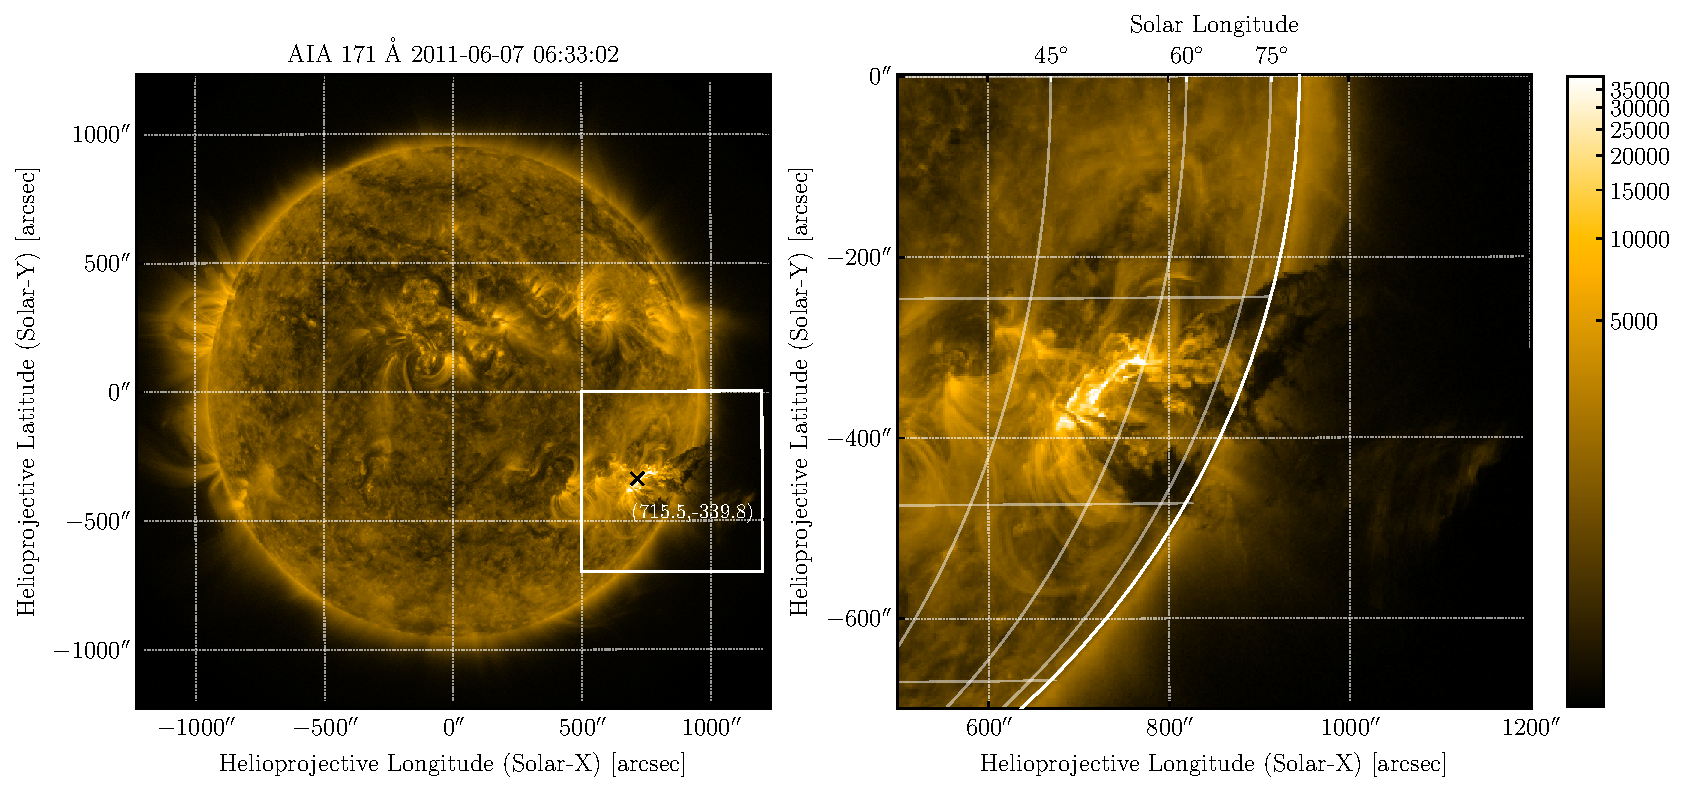
\includegraphics[width=0.97\textwidth]{figures/map_example.pdf}
    \caption{An example of a \Map visualization from observations of the 171~\AA\ wavelength channel of AIA aboard SDO.
    The left panel shows an image of the entire Sun with the flare position as given by the HEK. The right panel shows the cropped view in the white box of the left hand panel, focusing on an erupting flare (the same event as depicted in \autoref{fig:timeseries_example}).}
    \label{fig:map_example}
\end{figure}

The \Map class also provides functionality to analyze multiple images, such as overlaying images from different instruments with overlapping fields of view, or to combine multiple images together in a time-ordered sequence.
This class includes the ability to co-align images from different instruments or images taken at different times to facilitate multi-instrument studies.


\begin{figure}
    \center
    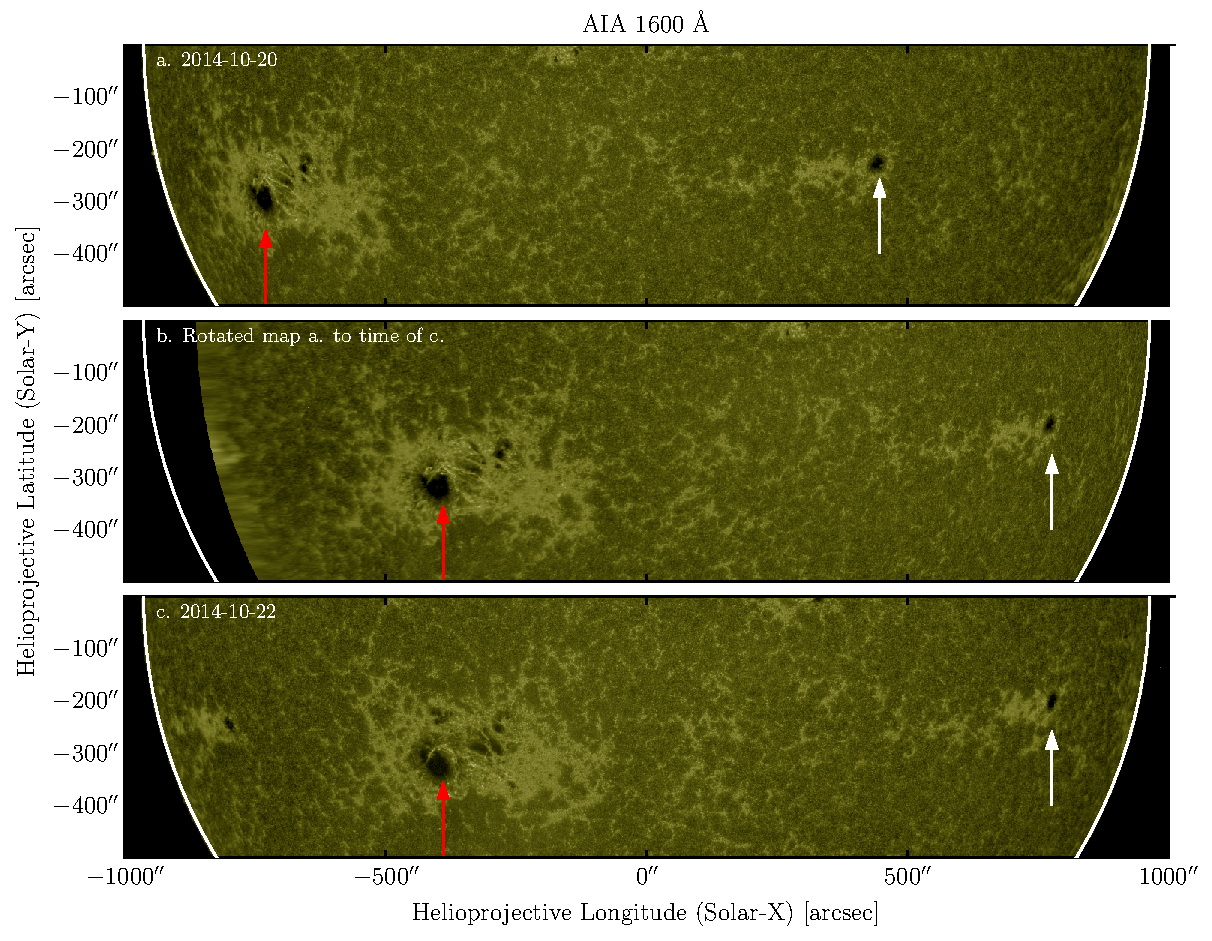
\includegraphics[width = 0.8\textwidth]{figures/fig_diff_rot_1600.pdf}
    \caption{An example of transforming a \Map to a different time, while accounting for differential rotation of the Sun.
    Panel (a) shows the Sun as observed by SDO AIA in 1600~\AA{} on a particular day.
    A large and small sunspot group are highlighted by a red arrow and a white arrow, respectively.
    Panel (b) shows the observation after transforming forward in time by two days.
    Panel (c) shows the real observation at the time of panel (b), which compares well to the transformed image, disregarding the magnetic evolution of the sunspot groups.}
    \label{fig:diff_rot}
\end{figure}

\Map currently supports the data sources listed in \autoref{tab:instruments} as well as the Helioviewer JPEG2000 image files of  each of these data sources.
Similar to \Timeseries, \Map is architected to enable new data sources to be added easily.
